\chapter{Primal Formulation with Linear Model}\label{chap: linear}

In the previous chapter, we introduced the general framework for binary classification at the top. Table~\ref{tab: summary formulations} summarizes all formulations that fall into this framework. In this chapter, we focus on the particular case when the model~$f$ is linear, i.e., the model is in the following form
\begin{equation*}
  f(\bm{x}; \bm{w}) = \bm{w}^{\top} \bm{x},
\end{equation*}
where~$\bm{w} \in \R^d$ is the normal vector to the separating hyperplane. In such a case, framework~\eqref{eq: aatp surrogate} simplifies into the form below
\begin{mini*}{\bm{w}, \, t}{
  \frac{1}{2} \norm{\bm{w}}^2 + \lambda_1 \cdot \fps(\bm{s}, t) + \lambda_2 \cdot \fns(\bm{s}, t)
  }{}{}
  \addConstraint{s_i}{= \bm{w}^{\top} \bm{x}_i, \quad i \in \I}
  \addConstraint{t}{= G\Brac{\bm{s}, \bm{y}}.}
\end{mini*}
In the upcoming sections, we provide a theoretical analysis of this unified framework with linear model. Moreover, we consider the problem formulations as derived in Chapter~\ref{chap: framework} and not individual algorithms which specify how to solve these formulations. The theoretical properties we mainly focus on are as follows:
\begin{itemize}
  \item \textit{Convexity} implies a guaranteed convergence for many optimization algorithms or their better convergence rates~\cite{boyd2004convex}.
  \item \textit{Differentiability} increases the speed of convergence.
  \item \textit{Stability} is a general term, by which we mean that the global minimum is not at~$\bm{w} = \bm{0}$. This actually happens for many formulations from Table~\ref{tab: summary formulations} and results in the situation where the separating hyperplane is degenerate and does not actually exist.
\end{itemize}
We show the results only for formulations from Section~\ref{sec: ranking} and~\ref{sec: aatp} for better readability. Formulations in Section~\ref{sec: aatp} are almost identical to the ones from Section~\ref{sec: Neyman-Pearson}. The only difference is that all formulations in Section~\ref{sec: aatp} compute the decision threshold from all samples, while formulations in Section~\ref{sec: Neyman-Pearson} use only negative samples. Therefore, the results for both sections are identical, and we show only the ones for Section~\ref{sec: aatp}. 

\section{Convexity}\label{sec: convexity}

Convexity is one of the most important properties in numerical optimization. It ensures that the optimization problem has neither stationary points nor local minima. All points of interest are global minima. Moreover, it allows for faster convergence rates. This section shows that some of the formulations from Table~\ref{tab: summary formulations} are convex and, therefore, easier to solve. The first result is summarized in the following proposition. Note that we denote the thresholds as functions of weights~$\bm{w}.$ This dependence holds since the thresholds are defined in Section~\ref{sec: aatp} as functions of scores~$\bm{s}.$

\begin{restatable}{proposition}{propconvex}\label{prop: convexity}
  Consider vector of scores~$\bm{s}$ with elements defined as~$s_i = \bm{w}^{\top} \bm{x}_i$ for all~$i \in \I$ and Notation~\ref{not: scores}. Recall the decision thresholds from Section~\ref{sec: ranking} and~\ref{sec: aatp} 
  \begin{align*}
    t_0(\bm{w}) &
      = s_{[1]}^-, &
    t_1(\bm{w}) &
      = \max \Set{t}{\frac{1}{n} \sum_{i \in \I} \Iverson{s_i \geq t} \geq \tau}, \\
    t_2(\bm{w}) &
      = \frac{1}{K} \sum_{i=1}^{K} s_{[i]}, &
    t_3(\bm{w}) &
      \quad \text{solves} \quad \frac{1}{n} \sum_{i \in \I} l\Brac{\vartheta(s_i - t)} = \tau,
  \end{align*}
  Then thresholds~$t_0$, ~$t_2$ and~$t_3$ are convex functions of weights~$\bm{w},$ while the threshold~$t_1$ is non-convex.
\end{restatable}

The proposition says that \Grill formulation uses non-convex threshold while \TopPush, \TopMeanK, and \PatMat use the convex ones. Moreover, the thresholds for \tauFPL and \TopPushK are convex since both formulations use almost the same threshold as \TopMeanK. The same holds for the thresholds of \PatMat and \PatMatNP formulations. Notice that all formulations that have a convex threshold use the same objective function.

\begin{restatable}{theorem}{thmconvex}\label{thm: convexity}
  If the threshold~$t = t(\bm{w})$ is a convex function of weights~$\bm{w}$, then function
  \begin{equation*}
    L(\bm{w}) = \fns(\bm{s}, t)
  \end{equation*}
  is convex.
\end{restatable}

While the proof of Theorem~\ref{thm: convexity} is simple, it points to the necessity of considering only false-negatives in the objective function. Due to this theorem, almost all formulations from Table~\ref{tab: summary formulations} are convex optimization problems. There are only two exceptions: \Grill and \GrillNP are not convex problems.

\section{Differentiability}

Similar to convexity, differentiability is crucial for improving the convergence rate. Moreover, differentiability can often be used to derive better termination criteria for numerical algorithms. The next theorem shows which formulations from Table~\ref{tab: summary formulations} are differentiable.

\begin{restatable}{theorem}{derivative}\label{thm: differentiability}
  Consider thresholds from Proposition~\ref{prop: convexity}.  Threshold~$t_0,$~$t_1$ and~$t_2$ are non-differentiable functions of weights~$\bm{w}.$ Moreover, if the surrogate function~$l$ is differentiable, threshold~$t_3$ is a differentiable function of weights~$\bm{w},$ and its derivative equals
  \begin{equation*}
    \nabla t_3(\bm{w}) = \frac{
      \sum_{i \in \I} l'\Brac{\vartheta (\bm{w}^{\top} \bm{x}_i - t_3(\bm{w}))}\bm{x}_i
      }{
        \sum_{j \in \I} l'\Brac{\vartheta (\bm{w}^{\top} \bm{x}_j - t_3(\bm{w}))}
      }.
  \end{equation*}
\end{restatable}

Due to the previous theorem and Theorem~\ref{thm: convexity}, only \PatMat, and \PatMatNP are convex and differentiable optimization problems. These properties allow us to prove the convergence of the stochastic gradient descent for these two formulations, as shown in Section~\ref{sec:convergence}.

\section{Stability}\label{sec: stability}

We first provide a simple example and show that many formulations from Table~\ref{tab: summary formulations} are degenerate for it. Then we analyze general conditions under which this degenerate behavior happens.

\begin{restatable}[Degenerate Behaviour]{example}{degeneratebehavior}\label{ex: degenerate behaviour}
  Consider~$n$ negative samples uniformly distributed in~$[-1,0]\times[-1,1]$,~$n$ positive samples uniformly distributed in~$[0,1]\times[-1,1]$ and one negative sample at~$(2,0).$ An illustration of such settings is provided in Figure~\ref{fig: degenerate behaviour} (\textbf{left}). If~$n$ is large enough, the point at~$(2,0),$ is an outlier and the problem is (almost) perfectly separable using the separating hyperplane with normal vector~$\bm{w}_1 = (1, 0)$. 
\end{restatable}

There are two important solutions for Example~\ref{ex: degenerate behaviour}. The first is the optimal solution~$\bm{w}_1=(1,0),$ which generates the optimal separating hyperplane. The second is~$\bm{w}_0=(0,0),$ a degenerate solution that does not generate any separating hyperplane. Since the dataset is perfectly separable by $\bm{w}_1$, we expect that~$\bm{w}_1$ provides a lower value of the objective function than~$\bm{w}_0$ for all formulations from Table~\ref{tab: summary formulations}. However, it is not happening. Table~\ref{tab: example} shows the threshold~$t$ and the value of the objective function~$L$ for~$\bm{w}_0$ and~$\bm{w}_1.$ For the precise computation of the results, see Appendix~\ref{app: stability}. By highlighting the better objective in Table~\ref{tab: example} by green, we see that \TopPush and \TopMeanK has a better objective in~$\bm{w}_0.$ It can be shown that~$\bm{w}_0$ is even the global minimum for these two formulations. This situation raises whether some tricks, such as early stopping or excluding a small ball around zero, cannot overcome this difficulty. The answer is negative, as shown in Figure~\ref{fig: degenerate behaviour} (\textbf{right}). Here, we run \TopPush with hinge loss as a surrogate and no regularization from several starting points. In all cases, \TopPush converges to zero from one of the three possible directions, and all these directions are far from the normal vector to the separating hyperplane.

\begin{figure}
  \centering
  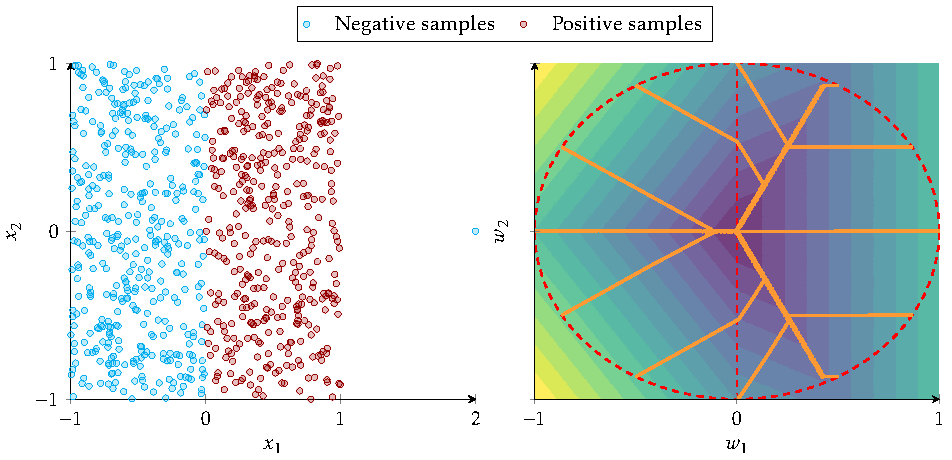
\includegraphics[width=\linewidth]{images/toppush_convergence.pdf}
  \caption{Distribution of positive (red circles) and negative samples (blue circles) for the example from Example~\ref{ex: degenerate behaviour}. (\textbf{left}) Contour plot of the objective function value for \TopPush with hinge loss as a surrogate and no regularization and its convergence (orange lines) to the zero vector from~$12$ different initial points. (\textbf{right})}
  \label{fig: degenerate behaviour}
\end{figure}

\begin{table}
  \centering
  \begin{NiceTabular}{lccccc}
    \CodeBefore
      \rowcolor{\headercol}{1-2}
      \rowcolors{4}{\rowcol}{}[restart]
    \Body
    \toprule
    \Block[c]{2-1}{\textbf{Formulation}}
      & \Block{2-1}{\textbf{Label}}
      & \Block{1-2}{$\bm{w}_0=(0,0)$}
      && \Block{1-2}{$\bm{w}_1=(1,0)$} \\
    \cline{3-6}
    & & $t$
      & $L$
      & $t$
      & $L$ \\
    \midrule
    \TopPush
      & \eqref{eq: toppush surrogate}
      & $0$
      & \Block[fill=mygreen!50]{1-1}{$1$}
      & $2$
      & $2.5$ \\
    \TopPushK
      & \eqref{eq: toppushK surrogate}
      & $0$
      & $1$
      & $\frac{2}{K}$
      & \Block[fill=mygreen!50]{1-1}{$0.5+\frac{2}{K}$} \\
    \midrule
    \Grill
      & \eqref{eq: grill}
      & $0$
      & $2$
      & $1-2\tau$
      & \Block[fill=mygreen!50]{1-1}{$1.5+2\tau(1-\tau)$} \\
    \TopMeanK
      & \eqref{eq: topmeank}
      & $0$
      & \Block[fill=mygreen!50]{1-1}{$1$}
      & $1-\tau$
      & $1.5-\tau$ \\
    \PatMat
      & \eqref{eq: patmat}
      & $\frac{1}{\vartheta}(1-\tau)$
      & $1+\frac{1}{\vartheta}(1-\tau)$
      & $\frac{1}{\vartheta}(1-\tau)$
      & \Block[fill=mygreen!50]{1-1}{$0.5 + \frac{1}{\vartheta}(1-\tau)$} \\
      \midrule
      \GrillNP
        & \eqref{eq: grill np}
        & $0$
        & $2$
        & $1-2\tau$
        & \Block[fill=mygreen!50]{1-1}{$1.5+2\tau(1-\tau)$} \\
      \tauFPL
        & \eqref{eq: tau-fpl}
        & $0$
        & \Block[fill=mygreen!50]{1-1}{$1$}
        & $1-\tau$
        & $1.5-\tau$ \\
      \PatMatNP
        & \eqref{eq: patmat np}
        & $\frac{1}{\vartheta}(1-\tau)$
        & $1+\frac{1}{\vartheta}(1-\tau)$
        & $\frac{1}{\vartheta}(1-\tau)$
        & \Block[fill=mygreen!50]{1-1}{$0.5 + \frac{1}{\vartheta}(1-\tau)$} \\
    \bottomrule
  \end{NiceTabular}
  \caption{Comparison of formulations from Table~\ref{tab: summary formulations} on the problem from Example~\ref{ex: degenerate behaviour}. The table shows the threshold and the objective function value for two solutions: the optimal solution~$\bm{w}_1=(1,0)$ and degenerate solution~$\bm{w}_0=(0,0).$ Three formulations have the global minimum (denoted by green color) at~$\bm{w}_0,$ which does not generate any separating hyperplane.}
  \label{tab: example}
\end{table}

The convexity derived in the previous section guarantees that there are no local minima. However, as we showed in the example above, the global minimum may be at~$\bm{w} = \bm{0}$. Such a situation is highly undesirable since~$\bm{w}$ is the normal vector to the separating hyperplane, and the zero vector provides no information. In the rest of the section, we analyze when this situation happens. The first result states that if the decision threshold~$t = t(\bm{w})$ is above a certain value, then zero has a better objective that~$\bm{w}$. If this happens for all~$\bm{w}$, then zero is the global minimum.

\begin{restatable}{theorem}{larget}\label{thm:large_t}
  Consider any of these formulations: \TopPush, \TopPushK, \TopMeanK or \tauFPL. Fix any~$\bm{w}$ and denote the corresponding objective function~$L(\bm{w})$ and threshold~$t(\bm{w})$. If we have
  \begin{equation}\label{eq:w_zero_nn}
    t(\bm{w})\geq \frac{1}{\npos} \sum_{i \in \Ipos} \bm{w}^{\top} \bm{x}_i,
  \end{equation}
  then~$L(\bm{0}) \leq L(\bm{w})$. Specifically, using notation~\ref{not: scores} we get the following implications
  \begin{align*}\label{eq:w_zero}
    s_{[1]}^- \geq \frac{1}{\npos} \sum_{i=1}^{\npos} s_{i}^+ \quad
      & \implies \quad L(\bm{0}) \leq L(\bm{w}) \text{ for } \TopPush, \\
    \frac{1}{K}\sum_{i=1}^K s_{[i]}^- \geq \frac{1}{\npos} \sum_{i=1}^{\npos} s_{i}^+  \quad
      & \implies \quad L(\bm{0}) \leq L(\bm{w}) \text{ for } \TopPushK, \\
    \frac{1}{K} \sum_{i=1}^{K} s_{[i]} \leq \sum_{i=1}^{\npos} s_{i}^+ \quad
      & \implies \quad L(\bm{0}) \leq L(\bm{w}) \text{ for } \TopMeanK, \\
    \frac{1}{\nneg\tau} \sum_{i=1}^{\nneg\tau} s_{[i]}^- \geq \frac{1}{\npos}\sum_{i=1}^{\npos} s_{i}^+ \quad
      & \implies \quad L(\bm{0}) \leq L(\bm{w}) \text{ for } \tauFPL. \\
  \end{align*}
\end{restatable}

The proof of Theorem~\ref{thm:large_t} employs the fact that all formulations in the theorem statement have only false-negatives in the objective. If we use the zero solution~$\bm{w}_0=\bm{0},$ all classification scores~$s_i$ are equal to zero, the threshold~$t$ equals zero, and the objective function~$L$ equals one. On the other hand, if the threshold~$t$ is large, many positive samples have scores below the threshold, and the false-negatives samples have the average surrogate value larger than one. In such a case,~$\bm{w}_0 = \bm{0}$ becomes the global minimum for some formulations. More specifically, \TopPush fails if there are outliers, and \TopMeanK fails whenever there are many positive samples.

\begin{corollary}\label{cor:toppush}
  Consider the \TopPush formulation. If positive samples lie in the convex hull of negative samples, then~$\bm{w}=\bm{0}$ is the global minimum.
\end{corollary}

\begin{corollary}\label{cor:topmean}
  Consider the \TopMeanK formulation. If~$\npos\geq n\tau$, then~$\bm{w}=\bm{0}$ is the global minimum.
\end{corollary}

There are two fixes to the situation described above:
\begin{itemize}
  \item Include false-positives to the objective. This approach is taken by \Grill and \GrillNP and necessarily results in the loss of convexity as shown in Section~\ref{sec: convexity}.
  \item Move the threshold away from zero even when all scores~$\bm{s}$ are zero. This approach is taken by our formulations \PatMat and \PatMatNP and keeps convexity.
\end{itemize}
The following theorem shows the advantage of the second approach.

\begin{restatable}{theorem}{patmatzero}\label{thm:patmat_zero}
  Consider the \PatMat or \PatMatNP formulation with the hinge loss as a surrogate and no regularization. Assume that for some~$\bm{w}$ we have
  \begin{equation}\label{eq:patmat_zero}
    \frac{1}{\npos}\sum_{i \in \Ipos}\bm{w}^{\top} \bm{x}_i > \frac{1}{\nneg}\sum_{j \in \Ineg}\bm{w}^{\top} \bm{x}_j.
  \end{equation}
  Then there exists a scaling parameter~$\vartheta_0$ for the surrogate top $\tau$-quantile~\eqref{eq: aatp quantile surrogate} or~\eqref{eq: np quantile surrogate} such that~$L(\bm{w}) < L(\bm{0})$ for all~$\vartheta \in (0, \vartheta_0)$.
\end{restatable}

This theorem shed some light on the behavior of the formulations. Theorem~\ref{thm:large_t} states that the stability of \tauFPL requires
\begin{equation}\label{eq:stability1}
  \frac{1}{\nneg\tau}\sum_{i=1}^{\nneg\tau}s_{[i]}^- < \frac{1}{\npos}\sum_{i=1}^{\npos} s_{i}^+,
\end{equation}
while Theorem~\ref{thm:patmat_zero} states that the stability of \PatMatNP is ensured by
\begin{equation}\label{eq:stability2}
  \frac{1}{\nneg}\sum_{i=1}^{\nneg}s_{[i]}^- < \frac{1}{\npos}\sum_{i=1}^{\npos} s_{i}^+.
\end{equation}
The right-hand sides of~\eqref{eq:stability1} and~\eqref{eq:stability2} are the same, while the left-hand side of~\eqref{eq:stability2} is always smaller than the left-hand side of~\eqref{eq:stability1}. This implies that if \tauFPL is stable, then \PatMatNP is stable as well.

At the same time, there may be a considerable difference in the stability of both formulations. Since the scores of positive samples should be above the scores of negative samples, the scores~$\bm{s}$ may be interpreted as performance. Then formula~\eqref{eq:stability1} states that if the mean performance of a \emph{small number of the best} negative samples is larger than the average performance of \emph{all} positive samples, then \tauFPL fails. On the other hand, formula~\eqref{eq:stability2} states that if the average performance of \emph{all} positive samples is better than the average performance of \emph{all} negative samples, then \PatMatNP is stable. The former may well happen as accuracy at the top is interested in a good performance of only a few positive samples.

\section{Convergence of stochastic gradient descent}\label{sec:convergence}

In the previous section, we analyzed the formulations from Table~\ref{tab: summary formulations}, but we did not consider any optimization algorithms. In this section we show a basic version of the stochastic gradient descent and then its convergent version. Due to considering the threshold, the gradient computed on a minibatch is a biased estimate of the true gradient. Therefore we need to use variance reduction techniques similar to SAG~\cite{schmidt2017minimizing}, and the proof is rather complex.

Many optimization algorithms for solving the formulations from Table~\ref{tab: summary formulations} use primal-dual or purely dual formulations. Authors of~\cite{eban2017scalable} introduced dual variables and used alternating optimization to the resulting min-max problem. In~\cite{li2014top, zhang2018tau}, authors dualized the problem and solved it with the steepest gradient ascent. Authors of~\cite{macha2020nonlinear} followed the same path but added kernels to handle non-linearity. We follow the ideas of~\cite{mackey2018constrained} and~\cite{adam2019machine} and solve the problems directly in their primal formulations. Therefore, even though we use the same formulation for \TopPush as~\cite{li2014top} or for \tauFPL as~\cite{zhang2018tau}, our solution process is different. However, both algorithms should converge to the same point due to convexity.

The decision variables in \eqref{eq: aatp surrogate} are the normal vector of the separating hyperplane~$\bm{w}$ and the threshold~$t$. To apply an efficient optimization method, we need to compute gradients. The simplest idea~\cite{grill2016learning} is to compute the gradient only with respect to~$\bm{w}$ and then recompute~$t$. A more sophisticated way is based on the chain rule. For each~$\bm{w}$, the threshold~$t$ can be computed uniquely. We stress this dependence by writing~$t(\bm{w})$ instead of~$t$. By doing so, we effectively remove the threshold~$t$ from the decision variables and~$\bm{w}$ remains the only decision variable. Note that the convexity is preserved. Then we can compute the derivative via the chain rule
\begin{equation}\label{eq:derivatives}
  \begin{aligned}
  L(\bm{w})
    & = \frac{1}{2}\norm{\bm{w}}^2 + \frac{1}{\npos} \sum_{i \in \Ipos} l(t(\bm{w}) - \bm{w}^{\top} \bm{x}_i) , \\
  \nabla L(\bm{w})
    & = \bm{w} + \frac{1}{\npos} \sum_{i \in \Ipos} l'(t(\bm{w}) - \bm{w}^{\top} \bm{x}_i)(\nabla t(\bm{w}) - \bm{x}_i).
  \end{aligned}
\end{equation}
The only remaining part is the computation of~$\nabla t(\bm{w})$. It is simple for most of the formulations from Table~\ref{tab: summary formulations}. Moreover, Theorem~\ref{thm: differentiability} shows the computation for \PatMat with efficient computation method presented in Appendix~\ref{app:threshold}. Having derivative \eqref{eq:derivatives}, deriving the stochastic gradient is simple. It partitions the dataset into minibatches and provides an update of the weights~$\bm{w}$ based only on a minibatch, namely by replacing the mean over the whole dataset in~\eqref{eq:derivatives} by a mean over the minibatch.

For the convergence proof of stochastic gradient descent, we need differentiability. Due to Theorem~\ref{thm: differentiability}, we have only two formulations that are differentiable: \PatMat and \PatMatNP. Therefore, in the rest of the section, we consider only these two formulations. Moreover, for simplicity, we show the proof only for \PatMat. At iteration~$k$ we have the decision variable~$\bm{w}^k$ and the active minibatch~$\Imb^k$. First, we update the vector of scores~$\bm{s}^k$ only on the active minibatch by setting
\begin{equation}\label{eq:defin_z}
  s_i^k = \begin{cases}
    \bm{x}_i^\top \bm{w}^k & \text{for all } i \in \Imb^k, \\
    s_i^{k-1} & \text{otherwise.}
  \end{cases} 
\end{equation}
We keep scores from previous minibatches intact. We use Appendix~\ref{app:threshold} to compute the surrogate quantile~$t^k$ as the unique solution of
\begin{equation}\label{eq:update_t}
  \sum_{i \in \I}l\Brac{\vartheta(s_i^k - t^k)} = n\tau.
\end{equation}
This is an approximation of the surrogate quantile~$t(\bm{w}^k)$ from \eqref{eq: aatp quantile surrogate}. The only difference from the true quantile is that we use delayed scores. Then we introduce artificial variable
\begin{equation}\label{eq:update_a}
  \bm{a}^k = \sum_{i \in \Imb^k} l'\Brac{\vartheta(s_i^k - t^k)}\bm{x}_i.
\end{equation}
Finally, we approximate the derivative~$\nabla f(\bm{w}^k)$ from \eqref{eq:derivatives} by
\begin{equation}\label{eq:update_g}
  g(\bm{w}^k)
    = \frac{1}{\nmbpos^k} \sum_{i \in \Imbpos^k} l'(t^k - s_i^k)(\nabla t^k - \bm{x}_i),
\end{equation}
where~$\nabla t^k$ is an approximation of~$\nabla t(\bm{w}^k)$ from Theorem~\ref{thm: differentiability} defined by
\begin{equation}\label{eq:update_nablat}
  \nabla t^k
    = \frac{\bm{a}^k + \bm{a}^{k-1} + \dots + \bm{a}^{k - m + 1}}{\sum_{i \in \I} l'\Brac{\vartheta(s_i^k - t^k)}}.
\end{equation}
A perhaps more straightforward possibility would be to consider only~$\bm{a}^k$ in the numerator of~\eqref{eq:update_nablat}. However, presented choice enables us to prove the convergence, and it adds stability to the algorithm for small minibatches. The whole procedure is summarized in Algorithm~\ref{alg:sgd}. Note that there are no vector operations outside of the current minibatch~$\Imb^k$. Moreover, note that a proper initialization for the first~$m$ iterations is needed.

\begin{restatable}{theorem}{sgd}\label{thm:sgd}
  Consider the \PatMat or \PatMatNP formulation, stepsizes~$\alpha^k = \nicefrac{\alpha^0}{k+1}$ and piecewise disjoint minibatches~$\Imb^1, \ldots, \; \Imb^m$ which cycle periodically~$\Imb^{k+m} = \Imb^k$. If~$l$ is the smoothened (Huberized) hinge function, then Algorithm~\ref{alg:sgd} converges to the global minimum of \eqref{eq: patmat}.
\end{restatable}

\begin{algorithm}
  \begin{algorithmic}[1]
    \Require Dataset~$\mathcal{D}$, minibatches~$\Imb^1,\; \Imb^2, \ldots, \; \Imb^m$, and stepsize~$\alpha^k$
    \State Initialize weights~$\bm{w}^0$
    \For{$k = 0, \; 1, \ldots $}
    \State Select a minibatch~$\Imb^k$
    \State Compute~$s_i^k$ for all~$i \in \Imb^k$ according to \eqref{eq:defin_z}
    \State Compute~$t^k$ according to \eqref{eq:update_t}
    \State Compute~$\bm{a}^k$ according to \eqref{eq:update_a}
    \State Compute~$\nabla t^k$ according to \eqref{eq:update_nablat}
    \State Compute~$g(\bm{w}^k)$ according to \eqref{eq:update_g}
    \State Set~$\bm{w}^{k+1} \gets \bm{w}^k - \alpha^k g(\bm{w}^k)$
    \EndFor
  \end{algorithmic}
  \caption{Stochastic gradient descent for \PatMat formulation}
  \label{alg:sgd}
\end{algorithm}

\pagebreak

\section{Summary}

In this chapter, we derived theoretical properties for formulations from Table~\ref{tab: summary formulations} with the linear model. We focused on the convexity, differentiability, and stability of formulations since these three properties are crucial for fast and proper convergence. All results are summarized in Table~\ref{tab: summary formulations properties linear}. We showed that \TopPush, \TopPushK, \TopMeanK, and \tauFPL are convex, but all these formulations are vulnerable to having the global minimum at~$\bm{w}=0$. On the other hand, Grill and \GrillNP are stable, but they are not convex or differentiable. Finally, our formulations \PatMat and \PatMatNP satisfy all three theoretical properties. 

A similar comparison is performed in Figure~\ref{fig:thresholds}. Methods in green and yellow are convex, while formulations in red are non-convex. Based on Theorem~\ref{thm:large_t}, four formulations in yellow are vulnerable to having the global minimum at~$\bm{w}=0$. This theorem states that the higher the threshold, the more vulnerable the formulation is. The full arrows depict this dependence. If it points from one formulation to another, the latter one has a smaller threshold and thus is less vulnerable to this undesired global minima. The dotted arrows indicate that this usually holds but not always. The precise formulation is provided in Appendix~\ref{app:relations}. This complies with Corollaries~\ref{cor:toppush} and~\ref{cor:topmean} which state that \TopPush and \TopMeanK are most vulnerable. At the same time, it says that \tauFPL is the best one from the yellow formulations. Finally, even though \PatMatNP has a worse approximation of the true threshold than \tauFPL due to Theorem~\ref{thm:large_t}, it is more stable due to the discussion after Theorem~\ref{thm:patmat_zero}.

\begin{table}
  \centering
  \begin{NiceTabular}{lccccc}
    \CodeBefore
      \rowcolor{\headercol}{1}
      \rowcolors{3}{\rowcol}{}[restart]
    \Body
    \toprule
    \Block[c]{1-1}{\textbf{Formulation}}
      & \textbf{Label}
      & \textbf{Hyperparameters}
      & \textbf{Convex}
      & \textbf{Differentiable}
      & \textbf{Stable} \\
    \midrule
    \TopPush
      & \eqref{eq: toppush surrogate}
      & ---
      & \yesmark
      & \nomark
      & \nomark \\
    \TopPushK
      & \eqref{eq: toppushK surrogate}
      & $K$
      & \yesmark
      & \nomark
      & \nomark \\
    \midrule
    \Grill
      & \eqref{eq: grill}
      & $\tau$
      & \nomark
      & \nomark
      & \yesmark \\
    \TopMeanK
      & \eqref{eq: topmeank}
      & $\tau$
      & \yesmark
      & \nomark
      & \nomark \\
    \PatMat
      & \eqref{eq: patmat}
      & $\tau$, $\vartheta$
      & \yesmark
      & \yesmark
      & \yesmark \\ 
    \midrule
    \GrillNP
      & \eqref{eq: grill np}
      & $\tau$
      & \nomark
      & \nomark
      & \yesmark \\
    \tauFPL
      & \eqref{eq: tau-fpl}
      & $\tau$
      & \yesmark
      & \nomark
      & \nomark \\
    \PatMatNP
      & \eqref{eq: patmat np}
      & $\tau$, $\vartheta$
      & \yesmark
      & \yesmark
      & \yesmark \\
    \bottomrule
  \end{NiceTabular}
  \caption{Summary of the formulations from Table~\ref{tab: summary formulations}. The second column shows the hyperparameters available for each formulation. The last three columns show whether the formulation is differentiable, convex, and stable (in the sense of having global minimum in~$\bm{w}=\bm{0}$).}
  \label{tab: summary formulations properties linear}
\end{table}

\begin{figure}
  \centering
  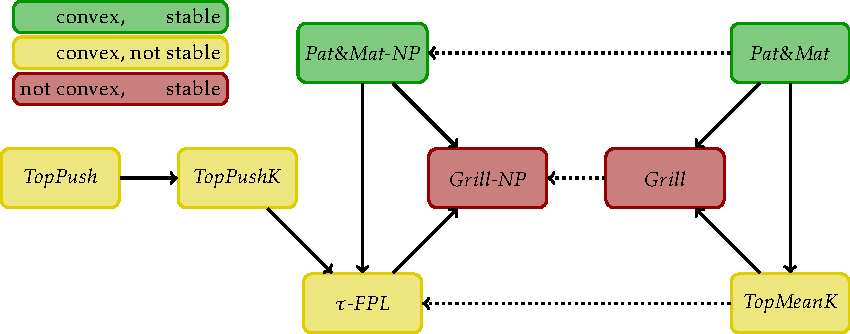
\includegraphics[width = \linewidth]{images/methods_relation.pdf}
  \caption{Summary of the formulations from Table~\ref{tab: summary formulations}. Methods in green and yellow are convex, while formulations in red are non-convex. Moreover, methods in yellow are vulnerable to having the global minimum at~$\bm{w}=0$. A full (dotted) arrow pointing from one formulation to another shows that the latter formulation has (usually) a smaller threshold.}
  \label{fig:thresholds}
\end{figure}